\section{Dinics}

\subsection{Sequential Algorithm}
    \subsubsection{Introduction}
    Dinic's algorithm is a flow algorithm that was created by Dr. Yefim Dinitz, and is notable for being strongly polynomial with an $\mathcal{O}(V^2E)$ run-time. Dinic's algorithm innovates on other flow algorithms with its use of level graphs and blocking flows. Dinic's algorithm uses BFS and DFS in order to achieve this superior run-time; bread-first search for building a level graph, and depth-first search with blocking flows in order to find the maximum flow efficiently.

    \subsubsection{Algorithm Overview}
       In what follows, we are going to walk the through the algorithm, step by step, with examples from our own implementation. \emph{To provide a brief overview of the original Dinic's algorithm, the pseudo-code has been provided below.}
       
    \begin{description}
        \item[] Input: A network G = ((V, E), c, s, t).
        \item[] Output: An s-t flow f of maximum value.  
    \end{description}    
    \begin{enumerate}
        \item Set $f(e) = 0$ for each $e \in E.$
        \item Construct $G_L$ from $G_f$ of G. If $dist(t)=\infty$, stop and output f.
        \item The text in the entries may be of any length.
    \end{enumerate}
    
    % \subsection{}
    The algorithm begins with the assumption that we want to make positive progress from the source node towards the sink node. We achieve this goal by using a level graph (Figure 11),
    
    \begin{figure}[H]
        \centering
        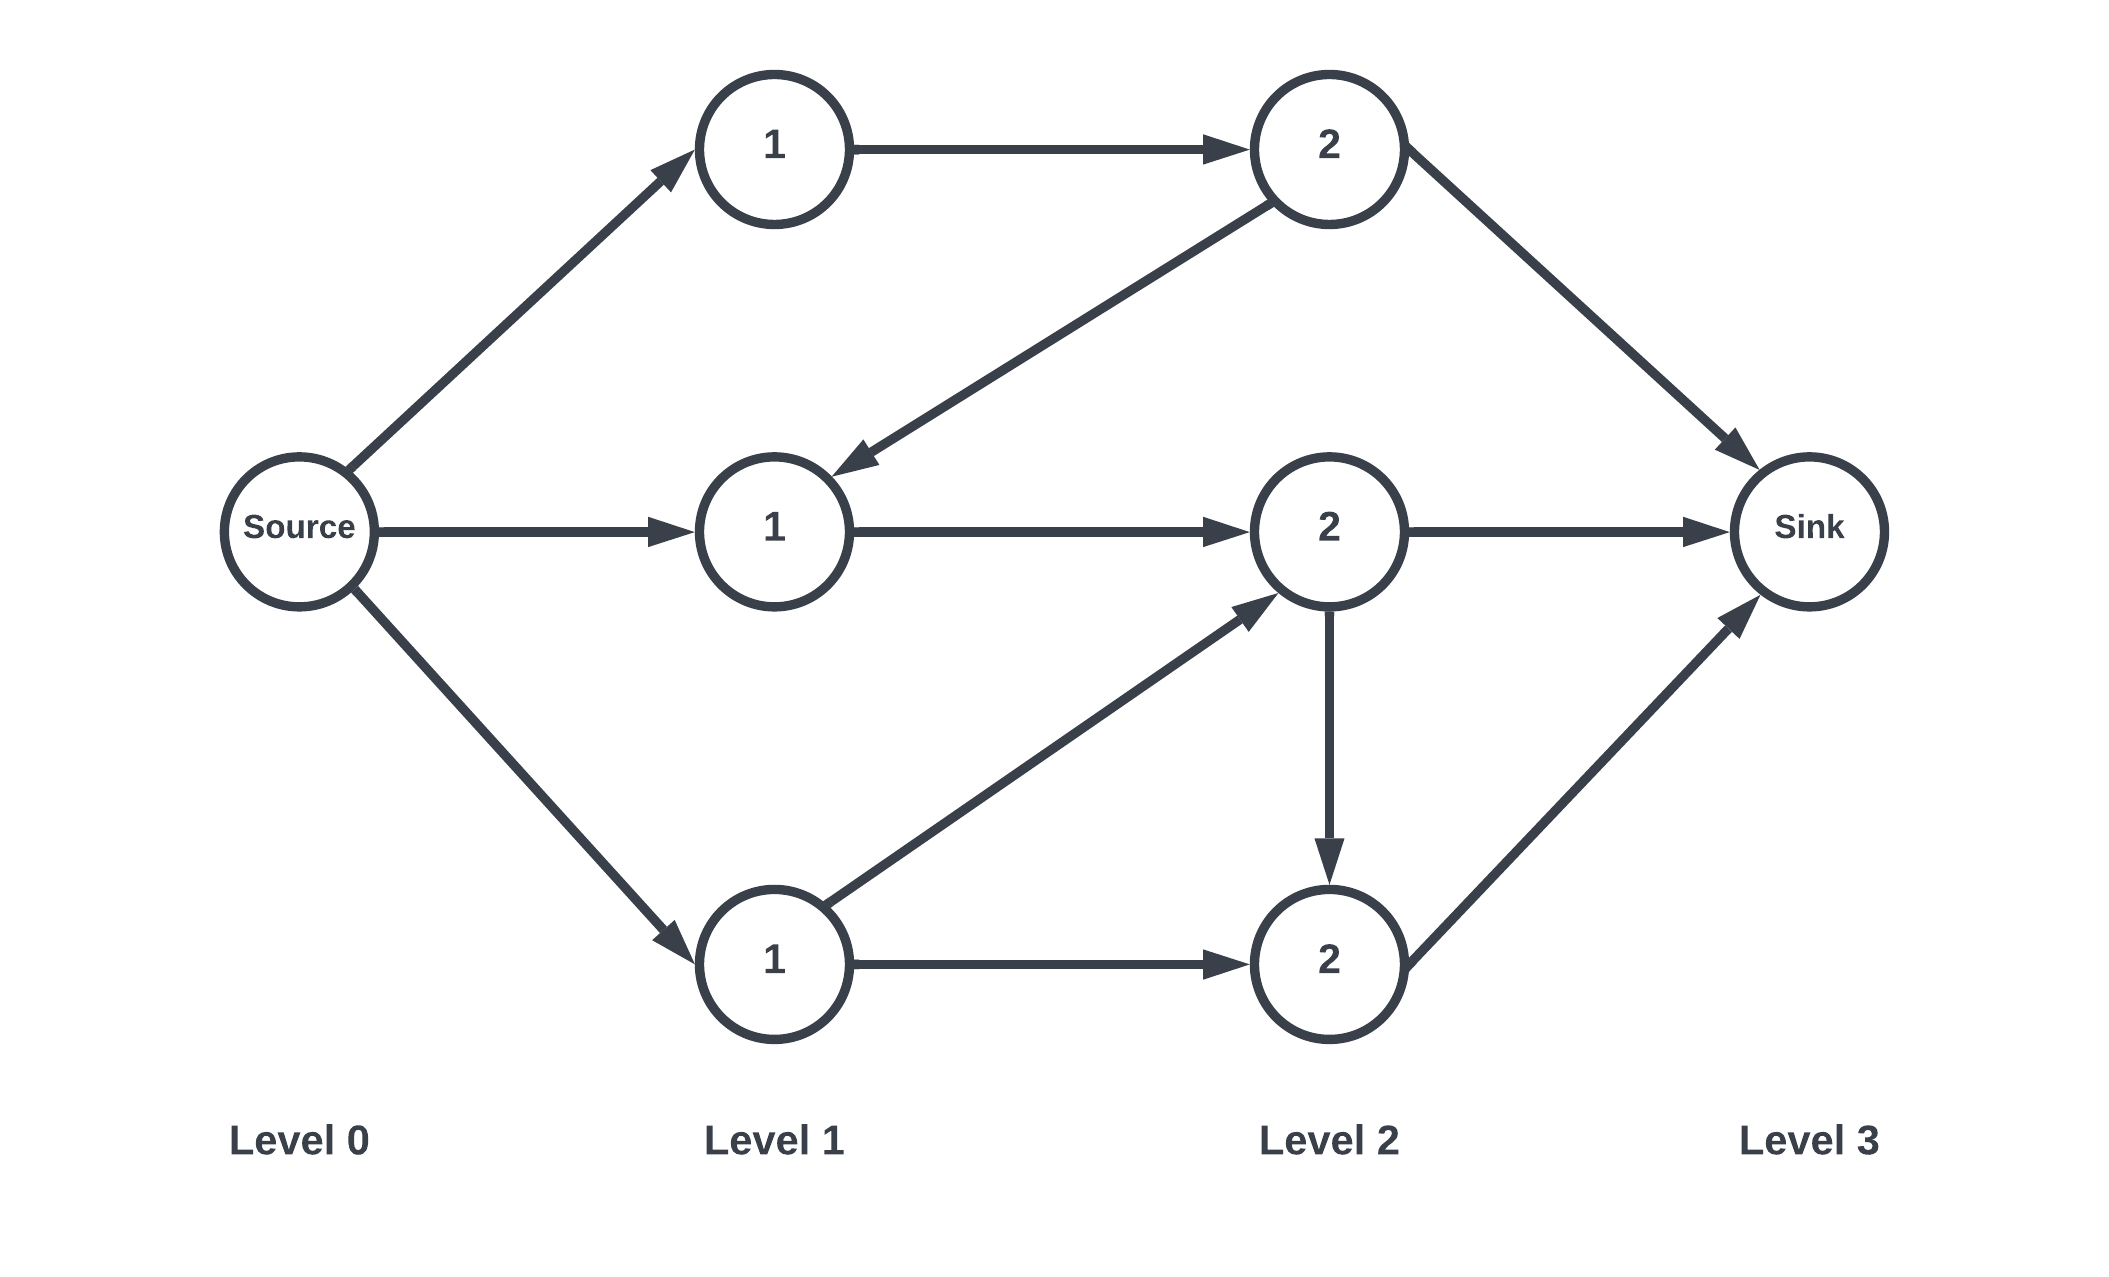
\includegraphics[scale=0.13, center]{figures/NetworkFlow_Dinics-4.png}
        \caption{Network Flow Graph}
    \end{figure}
    
    which keeps track of whether the edges are making progress towards the sink or not. This level graph is built using BFS, since with BFS we can easily calculate the minimum distance, or level, from the source node to other nodes. BFS achieves this by looking at the directed edges that point toward neighboring nodes from the current node, and if a level has not been set for those nodes, a level will be assigned. The neighboring nodes will get added to a queue for the next iteration of the BFS, where the same steps will take place, except this time, we will be setting the next set of neighboring nodes to level + 1. \cite{williamfiset} \emph{See pseudo-code below for a more detailed overview of how the Dinic's BFS would create a level graph:}
    
    \begin{algorithm}
        \caption{BFS Pseudo Code}
        \label{alg:BFS}
        \begin{algorithmic}[1]
            \State Node:
                \State $level \gets$ Integer
                \State $edges \gets$ Array of nodes\
                \State $capacityRemaining \gets$ Integer
                
            \Function{BFS}{} 
                \State $queue \gets$ empty queue of nodes\
                \State $queue \gets$ queue + source node\
                \State $level \gets$ 1\
                
                \While{queue is not empty} 
                    \For{for i in range 0, queue.size:}
                        \State $currentNode \gets$ queue.poll\
                        \State $neighbors \gets$findNeighbors(currentNode.edges)\
                        \For{neighbor in neighbors} 
                            \State $neighbor.level \gets$ level\
                            \State $queue \gets$ queue + neighbor\
                        \EndFor
                        \State $level \gets$ level + 1\
                    \EndFor
                \EndWhile
            \EndFunction    
            \\
            \Function{findNeighbors}{\var{edges}} 
                \State $neighbors \gets$ empty list of nodes\
                \For{neighbor in edges} 
                    \If {$neighbor.capacityRemaining > 0$ and level is not 0} 
                        \State $neighbors \gets$ neighbors + neighbor
                    \EndIf    
                \EndFor
                \State return neighbor
            \EndFunction
        \end{algorithmic}
    \end{algorithm}
            
    Once the level graph is completed using BFS, we are able to see if we're progressing forward by looking at whether the node level increases as we traverse the graph. Then we perform a DFS that looks for the paths from the source node to the sink node, filling up the capacity of the edges until we reach a "blocking flow". When we reach that point, we compute our max flow. We then repeat these steps until we reach a point where we can no longer keep going. \cite{Dinics-Fiset} 
    
\subsection{Parallel Algorithm}
    \subsubsection{Research}
        First, we decided to tackle parallelizing the BFS portion of Dinic's algorithm. A parallel BFS will allow for a concurrent construction of the level graph used in the algorithm \cite{pBFS}. To do this, we researched various ways in which standard BFS is parallelized; we noticed two possible approaches:
            \begin{enumerate}
                \item Using shared memory with a FIFO queue data structure.
                \item Using shared memory with a bag data structure.
            \end{enumerate}
        After extensive research, a few inherent issues with implementing a concurrent depth first search algorithm were discovered. The main issue being that depth first traversals follow sequential paths through a graph, going as deep as possible, before checking the neighboring nodes. This is perfect for augmenting flow in the Dinics algorithm, but poses a problem for our parallel implementation as threads may cross paths. To handle this, we decided to lock intersecting nodes, while waiting for a thread to finish sending blocking flow along a path, before unlocking the intersecting node to allow the previous to continue its traversal.
    \subsubsection{Final Approach}
        BFS: Since insertion and deletion from a queue both take $\mathcal{O}(1)$ time, while bags have an $\mathcal{O}(Log(N))$ worst case run time, we decided to implement the queue approach. We chose to spawn threads, or parallelize the task, at the point in which we enter the while loop in the BFS, which loops until the atomic queue is not empty. For each node that becomes available in the queue, a waiting thread will take that node, and compute the neighbors while adding them to the queue for the next available thread to process. \emph{See pseudo-code below for a more detailed overview:}
        
    \begin{algorithm} 
        \caption{Parallel BFS Pseudo Code}
        \label{alg:DParallel}
        \begin{algorithmic}[1]
            \State $runIndex(Atomic) \gets$ 0\
            \Function{Run}{}\
                \State $firstEntry \gets$ true\
                \While{firstEntry or runIndex is 0}
                    \State $firstEntry \gets$ false\
                    \State try:\
                        \State $runIndex \gets$ runIndex + 1\
                        \While{queue size is greater than 0}
                            \State $node \gets$ q.poll\
                            \For{each edge in graph[node]:}
                                \State $capacity \gets$ edge.remainingCapacity\
                                \If{capacity is greater than 0 and level[edge] == -1}
                                    \State $level[edge] \gets$ level[node] + 1\
                                    \State q.offer(edge)\
                                \EndIf
                            \EndFor
                        \EndWhile    
                    \State finally:\
                        \State $runIndex \gets$ runIndex - 1\
                \EndWhile        
            \EndFunction
        \end{algorithmic}
    \end{algorithm}     
    DFS: To implement our parallel DFS, we needed to handle the case when two threads encounter an intersecting node. This is due to the fact that if two threads have overlapping paths, that thread could be traveling down an invalid path, and in turn over-calculate the max flow. When two threads encounter the same node, one thread must wait until the other thread finishes sending blocking flow down its path. Once the thread has finished augmenting the edges, it can release the lock, allowing the waiting thread to continue. When the waiting thread begins to traverse the graph, it first checks to ensure there is still capacity along its edges as a safety guard against over-calculating the maximum flow. 
    
    The current implementation needs more research and development to ensure correctness as the graph grows in size, as well as how they perform on various platforms with varying number of threads. On certain platforms, with extremely large graphs, we observed unexpected results on 2 rare occasions. We currently hypothesize that this is due to traffic at intersecting nodes, or threads not traversing valid paths due to the current checking condition for a given path, both producing a max flow value that is slightly under calculated. These occurrences are rare, and only seen with 16 threads on an Apple M1 processor. Our results table was produced observing only correct output using 8 threads on UCF's eustis3 server. \emph{See pseudo-code below for a more detailed overview:}
  
    \begin{algorithm} 
        \caption{Parallel DFS Pseudo Code}
        \label{alg:DParallel}
        \begin{algorithmic}[1]
            \Function{Run}{}\
                \For{long f=dfs(source, next, INF); f!=o; f=dfs(source, next, INF)}
                    \State maxFlow += f\
                \EndFor        
            \EndFunction
            \\
            \Function{dfs}{} 
                \State $numEdges \gets$ Integer
                \State $edge \gets$ Edge
                \State $cap \gets$ Long
                \If{at == t}
                    \State flow\
                \EndIf                
                \State $numEdges \gets$ graph[at].size()\
                
                \For{; next[at]<numEdges; next[at]++} 
                    \If{$cap > 0$ \&\& level[edge.to] == level[at] + 1}
                        \State this.lock(edge.from)
                        \State try:\
                            \State $cap \gets$ edge.remainingCapacity()\
                            \If{$cap > 0$ \&\& level[edge.to] == level[at] + 1}
                                \State $bottleneck \gets$ dfs(edge.to, next, min(flow, cap))\
                                \If{$bottleneck > 0$}
                                    \State edge.augment(bottleneck)
                                    \State return bottleneck
                                \EndIf
                            \EndIf    
                        \State catch(Exception e)\
                            \State e.printStackTrace()  
                        \State finally:\
                            \State this.unlock(edge.from)                            
                    \EndIf             
                \EndFor
                \State return 0
            \EndFunction              
        \end{algorithmic}
    \end{algorithm}     
    
\subsection{Dinics Conclusion}
    The Dinics algorithm proved to be, by far, the fastest sequential algorithm out of the three we selected for this research paper, easily outperforming both Ford-Fulkerson and Edmonds-Karp. But due to the overhead with creating threads, as well as contention with threads fighting for progress at locked intersecting nodes in the DFS, we observed some speed-ups with a parallel BFS, but occasional slow-downs when using a parallel depth first search. We plan to look into further optimizations as we attempt to achieve further gains in efficiency, but this provides a solid foundation for further improvements in the area of parallelized network flow algorithms.

\subsection{Testing \& Results}
    These test results were performed on UCF's Eustis3 server utilizing open-source data sets.\\ \cite{sumitpadhiyar}
    
    The testing results show that the parallel DFS slows down the program compared to sequential with a 63.62\% decrease in speed when looking at the test case with 10,000 nodes. The parallel DFS+BFS slows down the program compared to sequential with a 48.28\% decrease in speed with the same test case. Meanwhile, the parallel BFS experienced a speedup of 13.21\% using that same test case (1.132 times faster). By Amdahl's Law, it can be determined that the parallel BFS program implementation of Dinics is 13.32\% concurrent.
    
    \newline
    \begin{figure}[H]
        \centering
        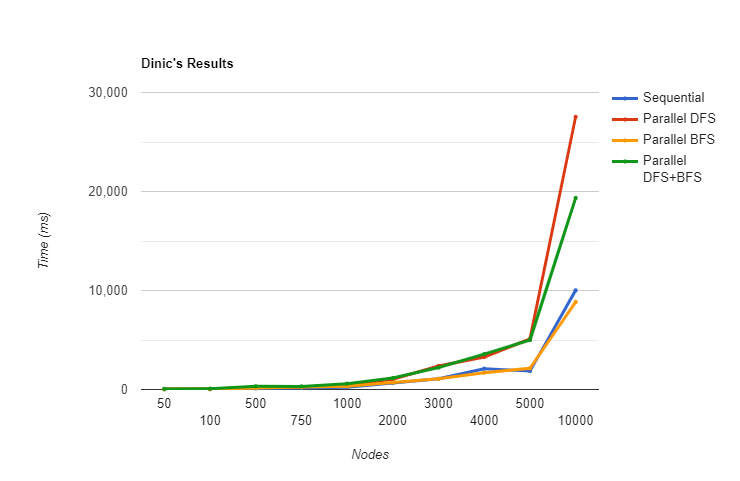
\includegraphics[scale=.36]{figures/line-graph_7.png}
        \label{fig:my_label}
    \end{figure}
    
    \begin{tabular}{ | m{2.3em} | m{2.5em }| m{3.8em} | m{3.2em} | m{3em} | m{3.9em} | } 
      \hline
      Nodes & Max Flow & Sequential Time & Parallel DFS Time & Parallel BFS Time & Parallel DFS+BFS Time\\
      
        \hline
        50      & 828     & 22ms & 54ms & 26ms & 59ms\\
        \hline
        100     & 1251    & 30ms & 53ms & 33ms & 86ms\\  
        \hline
        500     & 7143    & 104ms & 220ms & 144ms & 318ms\\        
        \hline   
        750     & 10930   & 164ms & 242ms & 242ms & 315ms \\         
        \hline
        1000    & 13476   & 232ms & 495ms & 320ms & 591ms \\          
        \hline
        2000    & 25027   & 650ms & 1035ms & 698ms & 1155ms \\      
        \hline
        3000    & 39170   & 1083ms & 2379ms & 1074ms & 2218ms \\            
        \hline
        4000    & 58517   & 2098ms & 3286ms & 1703ms & 3576ms \\      
        \hline
        5000    & 69349   & 1881ms & 5119ms & 2142ms & 4999ms \\      
        \hline
        10000   & 142610  & 10017ms & 27535ms & 8848ms & 19348ms \\      
        \hline
    \end{tabular}